% !TEX root = ../../mythesis.tex

\chapter{Background}
\label{chap:background}
    This chapter reviews the necessary background knowledge for the reader to be better acquainted with the work conducted within this thesis.
    It highlights the foundational technical basics of Ethereum blockchain, smart contracts, and the most common vulnerabilities associated with smart contracts.
    We cover these technicalities in the following order (based on the work of~\cite{ferreira2022smart}):
        First, we go over the basics of Ethereum, its components, and structure.
        We will go through how blocks are formed, what sort of accounts exist on the Ethereum network, and how transactions are executed.
        We will also go through how the Ethereum Virtual Machine functions.
        Afterward, we will go over smart contracts and their most common vulnerabilities out in the wild.
        We will discuss Solidity-written source code and bytecode of smart contracts and explain each vulnerability according to the DASP 10 classification.~\cite{dasp}


\section{Ethereum}
    Ethereum is a decentralized virtual machine introduced as alternative blockchain technology to Bitcoin in 2014 by~\cite{wood2014ethereum}.
    Blockchain are peer-to-peer networks made up of computers/nodes that update for one single global database without necessarily trusting in one another in a distributed fashion.
    It is based on a combination of cryptography, networking, and incentive mechanisms.~\cite{wohrer2018smart}
    The database mentioned above effectively serves as a ledger, recording every transaction that each node in the blockchain network makes. 


    \begin{figure}
        \centering
        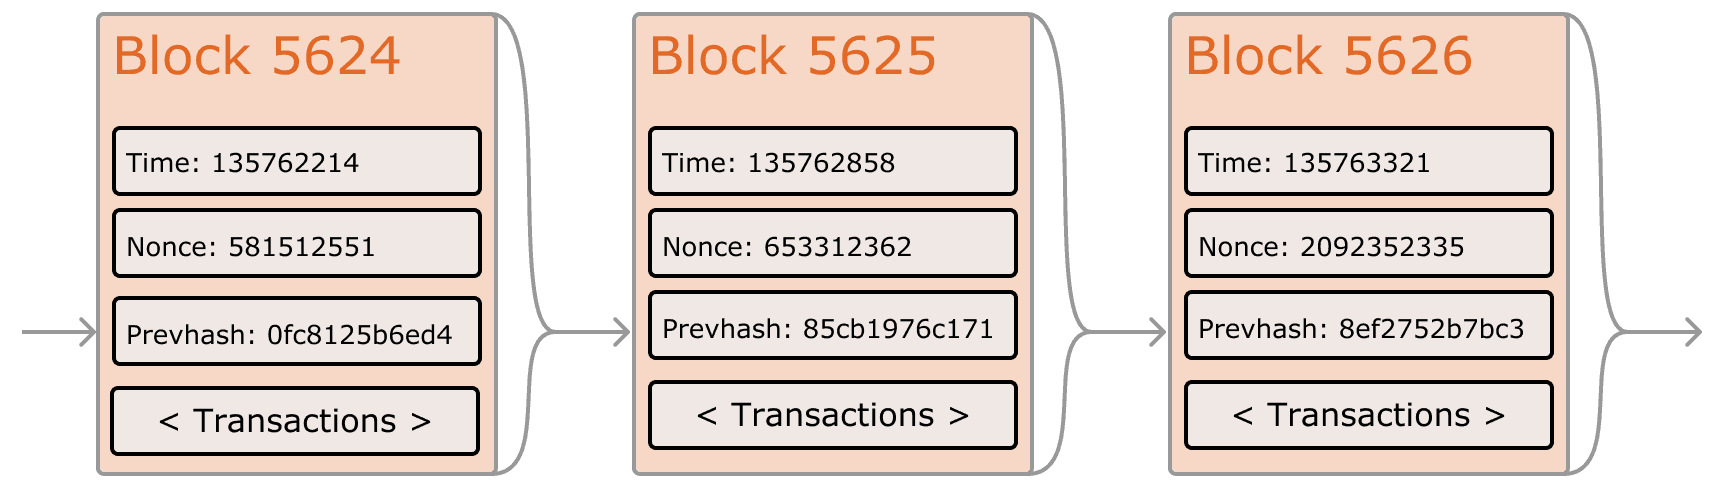
\includegraphics[width=\textwidth]{figures/ethereum-blocks.png}
        \caption{Ethereum blockchain structure.}
        \label{fig:ethereumBlockchainStructure}
    \end{figure}

    As the second most popular blockchain, the Ethereum blockchain is a transaction-based, cryptographically secure state machine.
    It takes a series of inputs transitions from its initial state to a new one according to the transition rules defined by those inputs.~\cite{ferreira2022smart}
    Like Bitcoin, Ethereum currently depends on the Proof-of-Work (PoW) consensus protocol.
    Proof-of-Stake (PoS) and PBFT(Practical Byzantine Fault Tolerance) are other forms of a consensus protocol, used by other blockchains per their defining characteristics.
    The PoW mechanism works as follows:
    A series of cryptographic puzzles aer intoroduced to the existing nodes on the network and the solutions to those puzzles are utilized as proof that the data being written on the blockchain are legitimate and credible.
    This gets verified through the concensus protocol.
    The puzzle is usually a computationally hard but easily verifiable mathematical problem.
    When a node creates a block, it must resolve a PoW puzzle and spend computing power to achieve so.
    Trying to solve the puzzles sooner than any other party, the nodes compete with each other over this objective function, and the node with the most computing power usually succeeds.
    After a node proves that their solution to a puzzle is correct, it will be broadcasted to other nodes so that all of them can reach concensus and agree upon appending a new block to the blockchain.~\cite{li2020survey}
    This acts as a proof that some node has done an amount of specific work to solve the puzzle by leveraging its computational resources.
    This whole process is called mining, and all the nodes participating in the process of competing with each other to create new blocks and append them to the blockchain are known as miners.

    \begin{figure}
        \centering
        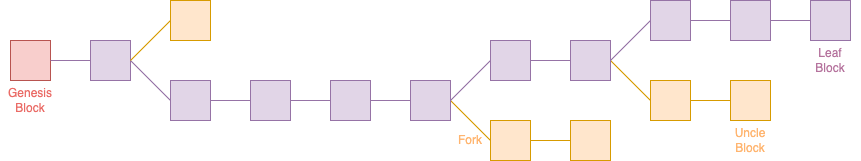
\includegraphics[width=\textwidth]{figures/uncle.png}
        \caption{Visualization of GHOST protocol in Ethereum.}
        \label{fig:uncle}
    \end{figure}

    \subsection{Accounts}
        The Ethereum state consists of many small objects named accounts.
        Each of these accounts are identified with a 20-byte address to interact with the other accounts on-chain.
        An address on the Ethereum blockchain is a 160-bit identifier used to identify any account.
        Ethereum supports two types of accounts:
        \begin{itemize}
            \item externally owned (controlled by private keys), known as EOAs, and
            \item contract accounts (CAs, controlled by their contract code).~\cite{ethereum2014ethereum}
        \end{itemize}
        *To Be Added*
        
        Inside of an Ethereum account is composed of four fields: nonce, ether balance, contract codeHash, and storageRoot, explained as follows:

        \begin{itemize}
            \item \textbf{Nonce:} Nonce counts the number of transactions sent from one address or the number of contract creations made by an account.
                                  Nonce is used to make sure that every transaction is processed once and only once.
                                  This is used to prevent replay attacks in Ethereum.
                                  Nonce counts the number of transactions initiated by the account to prevent replay attacks.
            \item \textbf{Balance:} (Ether) Balance basically records the Ethereum balance of the account, which is the amount of Wei assigned to the address of that account.
                                    Wei is the smallest measurement unit of Ether (1 Wei is the equivalent amount of 10-18 ethers).
            \item \textbf{storageRoot:} Each account has its own storage trie as explained above and StorageRoot is the 256-bit hash of the root node of a of that trie.
            \item \textbf{Contract codeHash:} The codeHash of a contract is the Keccak-256 hash value of the code of the account on the EVM.
        \end{itemize}

    \subsection{Transactions}
    A transaction is a cryptographically signed instruction sent by an account on the network towards another.
    There exist only two types of transactions based on the outcomes they generate:
    \begin{itemize}
        \item Message calls, which are created by contract accounts to produce and execute a message that leads to the recipient account (an EOA or contract account) running its code. The simplest of such transactions is sending Ether from one account to another.
        \item Contract creation call, which creates new accounts with a code associated with it.
    \end{itemize}
    

    \subsection{Ethereum Virtual Machine}
        The formal definition of the EVM is specified in the Ethereum Yellow Paper.~\cite{wood2014ethereum}
        The Ethereum Virtual Machine (EVM) at the heart of the Ethereum blockchain is a VM (virtual machine) with a stack-based architecture with 256-bit word sizes, supporting Turing-complete programming languages.
        EVM handles the computation side for Ethereum and comes with a set of instructions (namely, opcodes).
        Thus, a smart contract, from a low-level point of view, is a series of opcode instructions that EVM can read and compute and execute the logic of that smart contract.
        The EVM is also responsible for estimating and calculating gas consumption for transactions in smart contracts.


\section{Smart Contracts}
    Nick Szabo introduced smart contracts as a concept - programs running on the EVM - in one of his works in 1997.~\cite{szabo1997formalizing}
    They provide a framework that allows any sound program to be executed in an autonomous, distributed, and trusted manner.~\cite{nguyen2020sfuzz}
    The main programming language currently in use for the development of smart contracts is Solidity, although Vyper is gaining gradual traction as well.

    \subsection{Vulnerabilities}
        Solidity, like any other programming language in history, is prone to all kinds of vulnerabilities.
        What makes security vulnerabilities in Solidity so attractive is the fact that the programs written in Solidity are very often used in the financial sector,
        handling millions of dollars in digital assets and cryptocurrencies. Attacking such contracts successfully can result in enormous financial losses.
        Some of these vulnerabilities, like another programming language, arising from the human factor involved in the development of the smart contracts, and some are specific to the blockchain data structures and how they and their components function and interact with each other.
        Furthermore, these are only vulnerabilities within the scope of smart contracts we focus on. Vulnerabilities can arise regarding the blockchains' core infrastructure handling smart contracts.
        In this section, we go over 9 of the more discussed vulnerabilities in Solidity and Ethereum according to ~\cite{dasp} to get a better sense of what threat surface the developers and researchers developing analysis tools face:

            \paragraph{Reentrancy}
            Often called the most famous Ethereum vulnerability, the reentrancy attack has been a great example of showing the risks of \textit{"Code is Law"} and the importance of smart contract security historically.
            The DAO hack ~\cite{dhillon2017dao} is one of the most famous real-world examples of the reentrancy hack.
            The reentrancy attack can also be counted as a denial-of-service (DoS) attack, where a malicious actor can cause a program to infinitely loop and consume CPU cycles and, in the case of smart contracts, drain a wallet of its ETHs.
            The reentrancy vulnerability is exploited when external contract calls are allowed to make new calls to the calling contract before the initial execution of that call is complete.~\cite{dasp}

            \paragraph{Access Control}
            The Access Control vulnerability, not exclusive to smart contract types of programs, usually occurs when smart contracts use poor visibility settings regarding calling functions.
            This gives the attackers the ability to try to access the smart contract's private values or hijack the control of the smart contract (for example, becoming the owner of a contract by initializing that contract through a statement like \texttt{owner = msg.sender()}).

            \paragraph{Arithmetic}
            Integer overflows and underflows can cause huge losses in smart contract-based applications~\cite{arithmeticVuln}.
            Values assigned with the integer data type, if not handled carefully concerning being signed or unsigned integers, can cause overflows and underflows and cause DoS-type attacks.
            
            \paragraph{Unhandled Exception}
            Also known as unchecked-send, this vulnerability can cause unwanted outcomes when the smart contract is executed because some low-level calls in Solidity like \texttt{call()} and \texttt{delegatecall()} can return a boolean value set to the value False and lt the execution flow resume if an error happens mid-execution.
            This is not ideal since it means that the execution of the smart contract has not been reversed and successfully completed but with wrong or undesirable outcomes.
            Thus, the return values of such low-level calls should always be checked, and the developers must ensure that such exceptions are handled appropriately during execution.
            
            \paragraph{Frontrunning}
            The frontrunning vulnerability is one of the more famous ones in the list, also known as Transaction Ordering Dependence (TOD).
            Exploiting this vulnerability happens when malicious miners alter the initial default ordering of the transactions submitted to the blockchain.
            Per Eskandari et al.~\cite{eskandari2018frontrunning}, frontrunning can be generally reduced into three templates:
            \begin{itemize}
                \item Displacement attack, where an adversarial party makes a transaction in order to displace the victim user's transaction by having a higher gas price, and thus, the attacker's transaction gets mined before that of the victim's due to it giving having more aligned incentives with he miners' network.
                \item Insertion attack, in which an adversarial actor makes two transactions, one with a higher gas price than that of the victim and one with a lower gas price, to \textit{sandwich} the victim transaction.~\cite{varun2022mitigating}
                \item Suppression attack, where an attacker makes multiple transactions with higher gas prices than the victim transactions to prevent them from being mined in the same block.
            \end{itemize}

            \paragraph{Bad Randomness}
            Also known as \textit{nothing is secret},~\cite{dasp} this vulnerability happens when smart contracts attempt to generate random, or to be more exact, pseudo-random numbers for any number of reasons.
            If the smart contract generating the pseudo-random number computes that random number using values that a malicious party can guess, then the attacker can predict the next number that will be generated.
            Values such as block timestamps or block numbers are generally advised against being used in such mechanisms. They are called hard-to-predict values, but it is better to use an external oracle to generate the random numbers needed~\cite{swcregistry}.
        
            \paragraph{Time Manipulation}
            This vulnerability is also known as \textit{timestamp dependence}~\cite{dasp}.
            In Solidity, a block's timestamp is often used to generate pseudo-random numbers. In other times, it can be leveraged for smart contracts to conduct time-intensive operations, like unlocking funds at a specific time.
            A malicious miner of a block can manipulate the timestamp reported while generating the block and use this vulnerability for their profit. 
        
            \paragraph{Short Address}
            The short address vulnerability, also known as off-chain issues, results from the Ethereum Virtual Machine accepting arguments with incorrect paddings.
            Attackers exploiting this vulnerability can craft truncated addresses that clients may encode incorrectly in transactions.
            Additionally, it has not been exploited in the wild, as mentioned by ~\cite{ferreira2020smartbugs}.